\chapter{مقدمه}
\section{خوش آمدید}
هدف از نوشتن این کتاب، آشنایی خوانندگان محترم با توزیع گنو/لینوکس اوبونتو و همچنین پیش‌نیازهای کار با آن که عمدتاً برگرفته از توزیع دبیان است، می‌باشد. این کتاب با این هدف نوشته شده است که بتواند عمده نیازهای اولیه کاربران را بدون نیاز به مراجعه به دیگر منابع مرتبط با توزیع‌‌های دبیان یا اوبونتو برطرف نماید.
\section{اوبونتو چیست؟}
اوبونتو
\footnote{Ubuntu}
سیستم عاملی است شبه‌یونیکسی که از هسته‌ی لینوکس استفاده می‌کند.
\begin{figure}[hbtp]
\centering
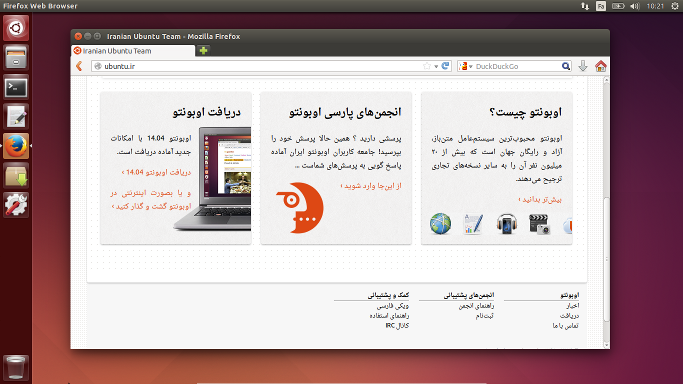
\includegraphics[scale=0.5]{pics/ubuntu-14.04-firefox.png}
\caption{اوبونتو ۱۴٫۰۴ در حال اجرای فایرفاکس}
\label{fig:ubuntu-14.04-firefox}
\end{figure}

\section{مطالعه‌ی بیشتر}